\documentclass{article}


\usepackage[letterpaper, margin=1in]{geometry}
\usepackage{amsmath}

\usepackage{fancyvrb} % verbatim replacement that allows latex
\DefineVerbatimEnvironment{Highlighting}{Verbatim}{commandchars=\\\{\}}

\usepackage{url}
% For basic math, align, fonts, etc.
\usepackage{amsmath}
\usepackage{amsthm}
\usepackage{amssymb}
\usepackage{mathtools}
\usepackage{mathrsfs}
\mathtoolsset{showonlyrefs}

\usepackage{hyperref}
\usepackage{siunitx}
\usepackage{float}
\usepackage{listings}

% For color
\usepackage{xcolor}
\definecolor{dark-red}{rgb}{0.4,0.15,0.15}
\definecolor{dark-blue}{rgb}{0,0,0.7}
\hypersetup{
    colorlinks, linkcolor={dark-blue},
    citecolor={dark-blue}, urlcolor={dark-blue}
}

\begin{document}
\section{Load Balancing Output}

\begin{figure}[H]
        \centering
        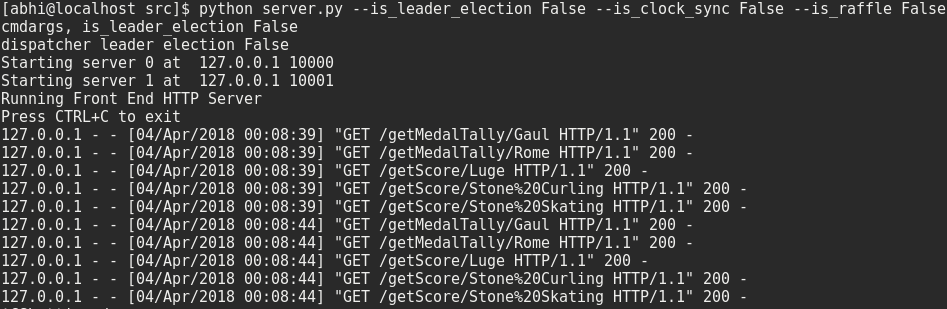
\includegraphics[width=\textwidth]{outputs/dispatcher.png}
        \caption{Dispatcher and server working}
\end{figure}

\begin{figure}[H]
        \centering
        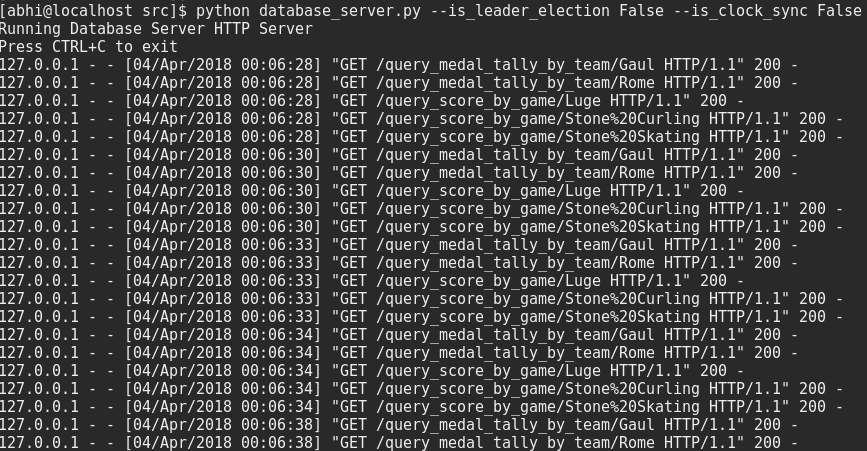
\includegraphics[width=\textwidth]{outputs/db_output.png}
        \caption{Database server working}
\end{figure}

\begin{figure}[H]
        \centering
        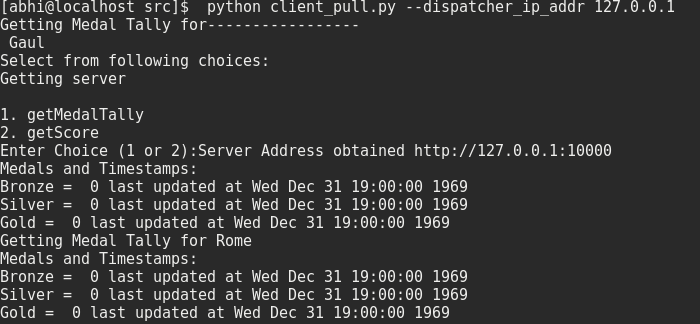
\includegraphics[width=\textwidth]{outputs/client_pull_server0.png}
        \caption{Client connected to server 0}
\end{figure}


\begin{figure}[H]
        \centering
        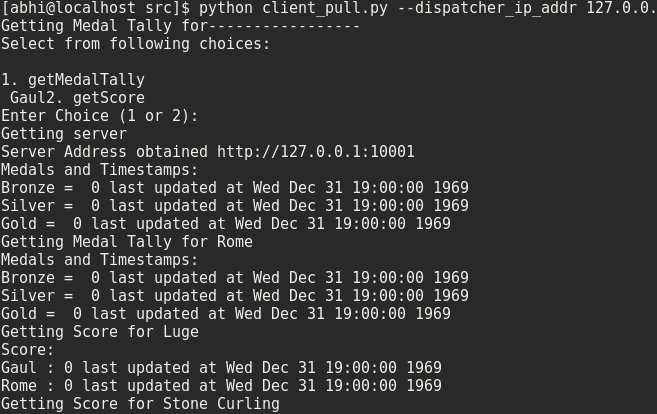
\includegraphics[width=\textwidth]{outputs/client_pull_server1.png}
        \caption{Client connected to server 1}
\end{figure}

\section{Raffle Winner Working}

\begin{figure}[H]
        \centering
        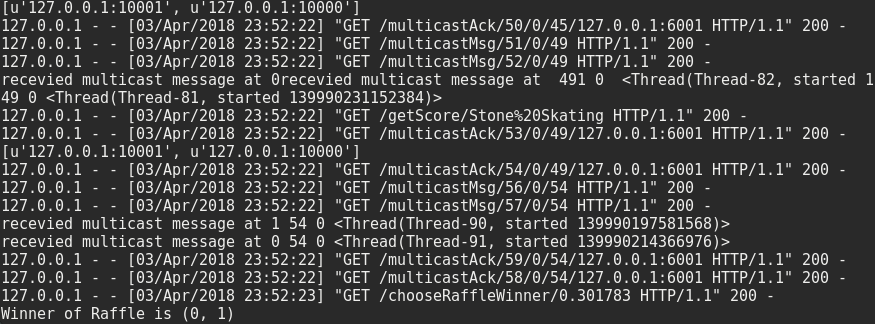
\includegraphics[width=\textwidth]{outputs/raffle_winner.png}
        \caption{Raffle Winner}
\end{figure}

\section{Clock Synchronization}
\begin{figure}[H]
        \centering
        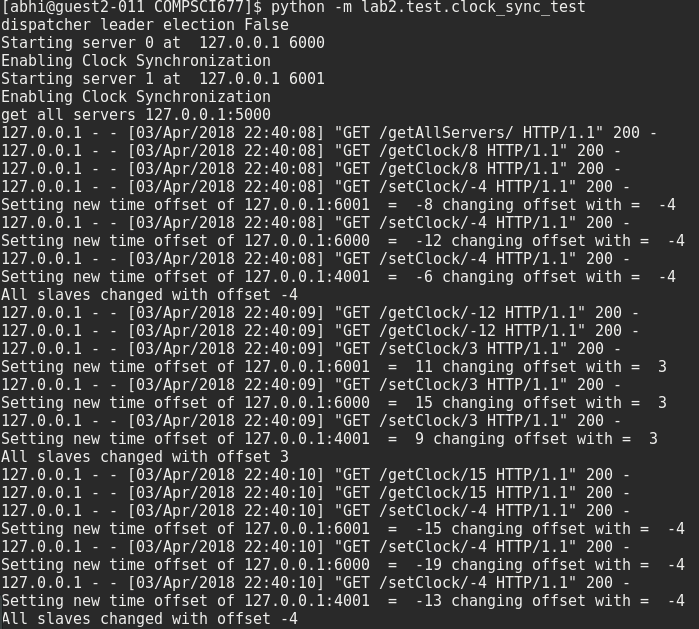
\includegraphics[width=\textwidth]{outputs/clock_sync_test_start.png}
        \caption{Clock Syncronization Start}
\end{figure}
\begin{figure}[H]
        \centering
        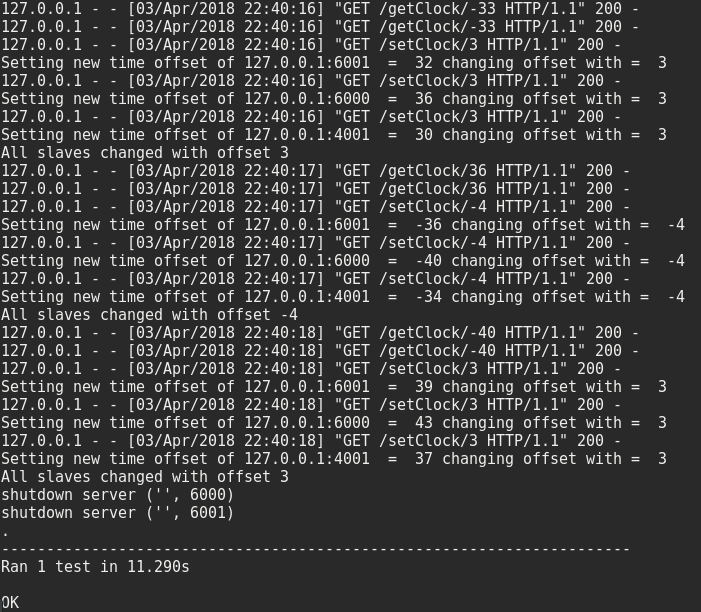
\includegraphics[width=\textwidth]{outputs/clock_sync_test_end.png}
        \caption{Clock Synchronization End}
\end{figure}

\section{Leader Election}
\begin{figure}[H]
        \centering
        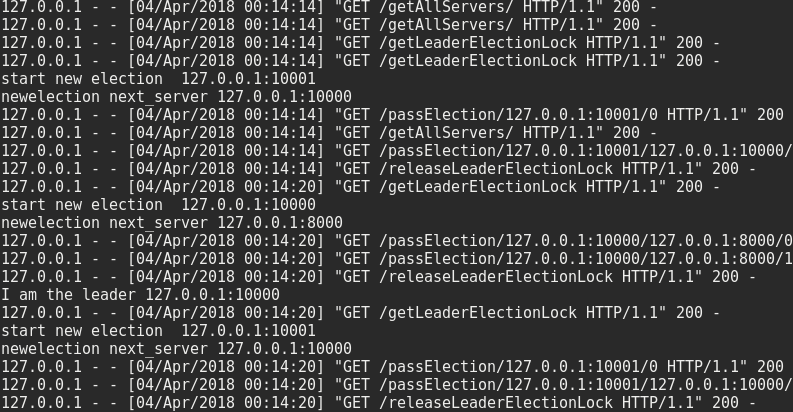
\includegraphics[width=\textwidth]{outputs/leader_election.png}
        \caption{Leader Election}
\end{figure}
\end{document}
